\begin{quote} \textit{1) Estudiar las corrientes y tensiones en todos los componentes en función del tiempo, desde que se enciende el regulador ($t=0$) hasta régimen permanente. En particular, en régimen permanente, estudiar en detalle las corrientes y tensiones en un intervalo de unos pocos periodos.}
\end{quote}

\HgraficarPNG{0.4}{fly}{Regulador \textit{Flyback} aislado.}{fig:cto}

En la Figura \ref{fig:cto} se muestra el circuito completo bajo análisis. Se trata de un regulador tipo \textit{Flyback} aislado utilizdo a nivel industrial ya que posee múltiples salidas y los componentes magnéticos que lo conforman son económicos.\\
\indent Para realizar un análisis cualitativo del mismo, se puede considerar el cirucito simplificado de la Figura \ref{fig:cto_simple}, donde se reemplazó el rectificador por una tensión constante, y sólo se consideró una de las salidas.

\HgraficarEPS{0.5}{fly_simple}{Circuito simplificado.}{fig:cto_simple}

\begin{itemize}
	\item \textcolor{blue}{\textbf{Primer ciclo:}} $V_{GS}=\SI{12}{\volt}$ (llave cerrada) el MOSFET se encuentra en conducción, por lo que $L_1$ se carga e induce una tensión en $L_2$, de polaridad inversa según la notación de los bornes homólogos. Esto hace que el diodo $D$ esté en inversa y por ende no circula corriente por la malla de $L_2$. En esta parte del ciclo ambos núcleos almacenan energía.

	\item \textcolor{red}{\textbf{Segundo ciclo:}} $V_{GS} = \SI{0}{\volt}$ (llave abierta) la tensión en $L_1$ se inveirte para contrarrestar el cambio abrupto de corriente, por lo que también se invierte la polaridad en $L_2$, pero la corriente en $L_1$ será nula por estar el MOSFET en corte.
		En este ciclo $L_2$ se descarga con el fin de cargar al capacitor $C_S$, el cuál se encarga de entregar la tensión de salida. A su vez se sabe que el circuito está operando en modo discontinuo, por lo que $L_2$ alcanza a descargase por completo en este ciclo.
\end{itemize}


Asimismo se debe destacar que $L_1$ y $L_2$ no conforman un transformador sino que son dos inductores porque no circula corriente por ambos inductores simultáneamente.


En la Figura \ref{fig:esq} se muestra el esquema de simulación, siendo las corrientes y tensiones más relevantes las que se muestran en \ref{fig:transitorio}{ y \ref{fig:permanente}.

\begin{figure}[H]
	\centering
	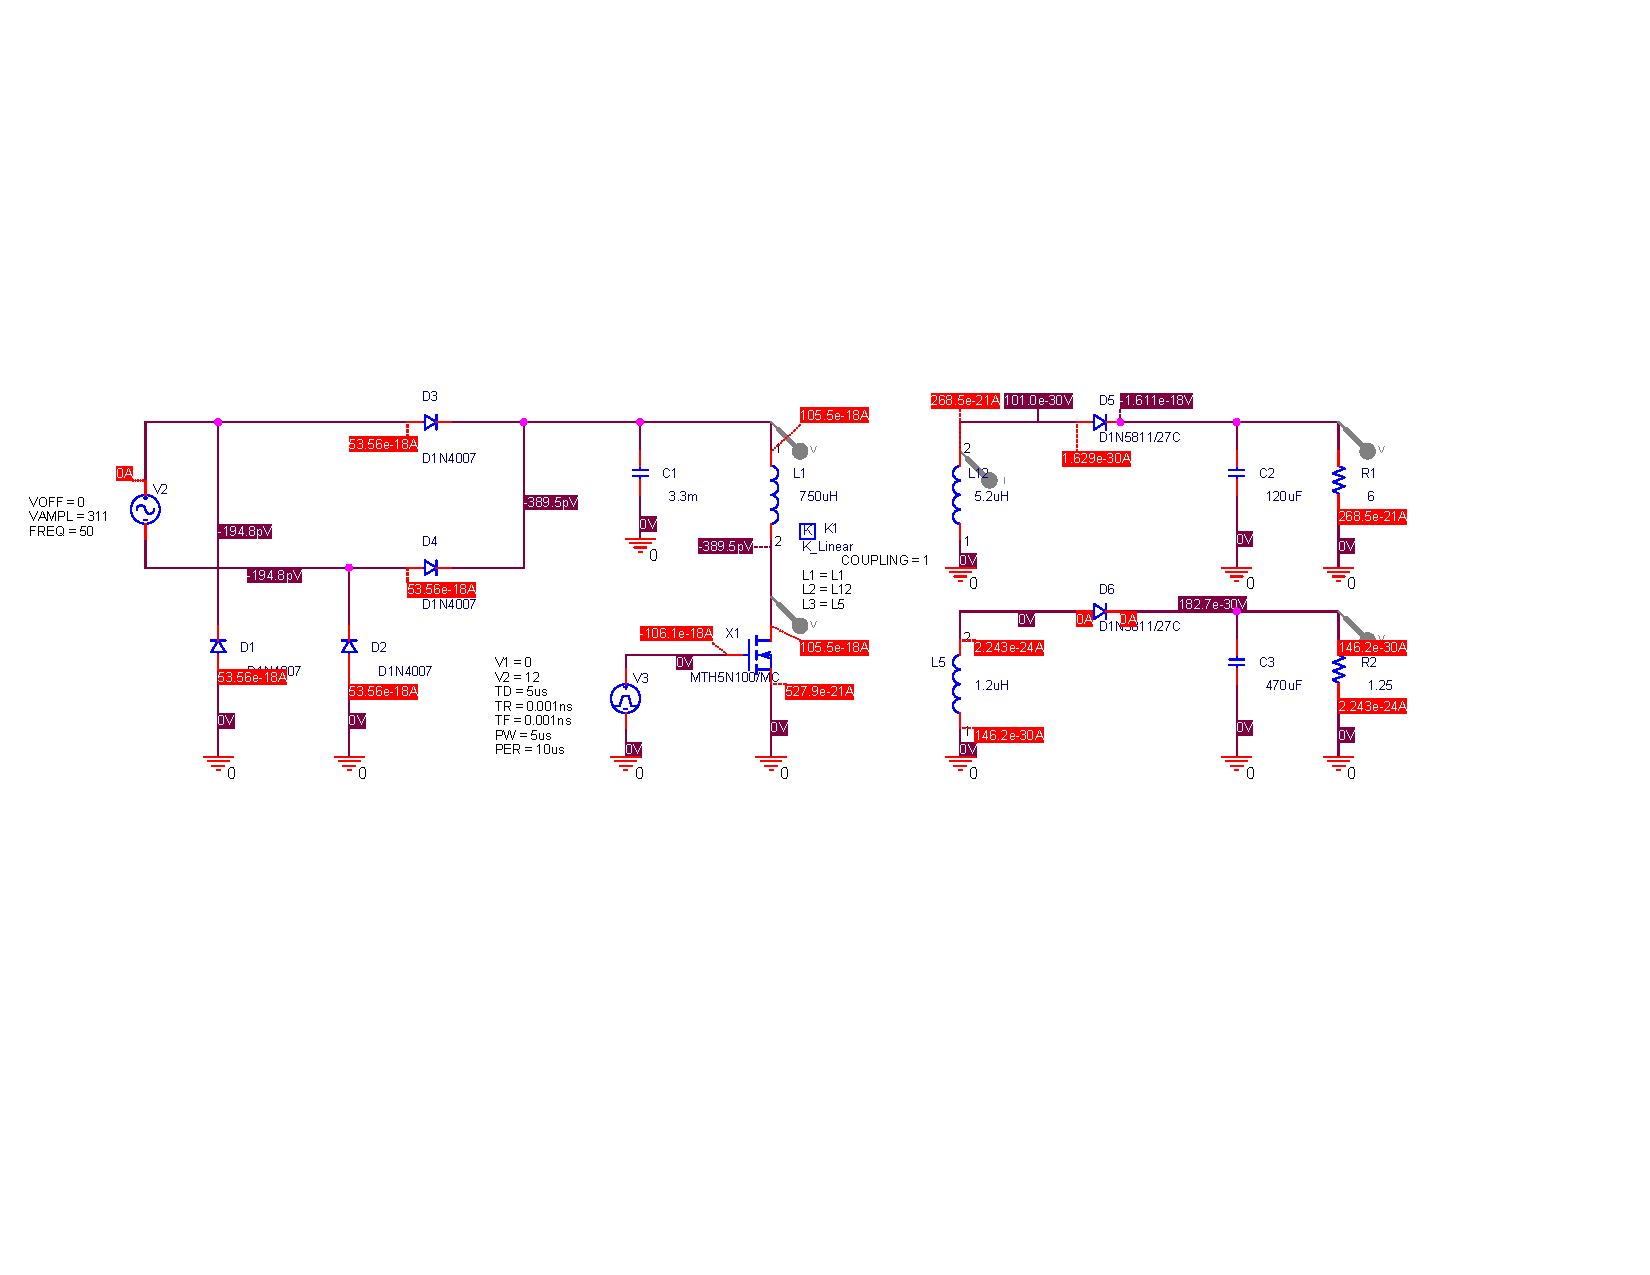
\includegraphics[scale=0.5]{Figuras/1_esquematico.pdf}
	\caption{Circuito bajo análisis con \textit{PSpice}.}
	\label{fig:esq}
\end{figure}


\begin{figure}[H]
	\centering
	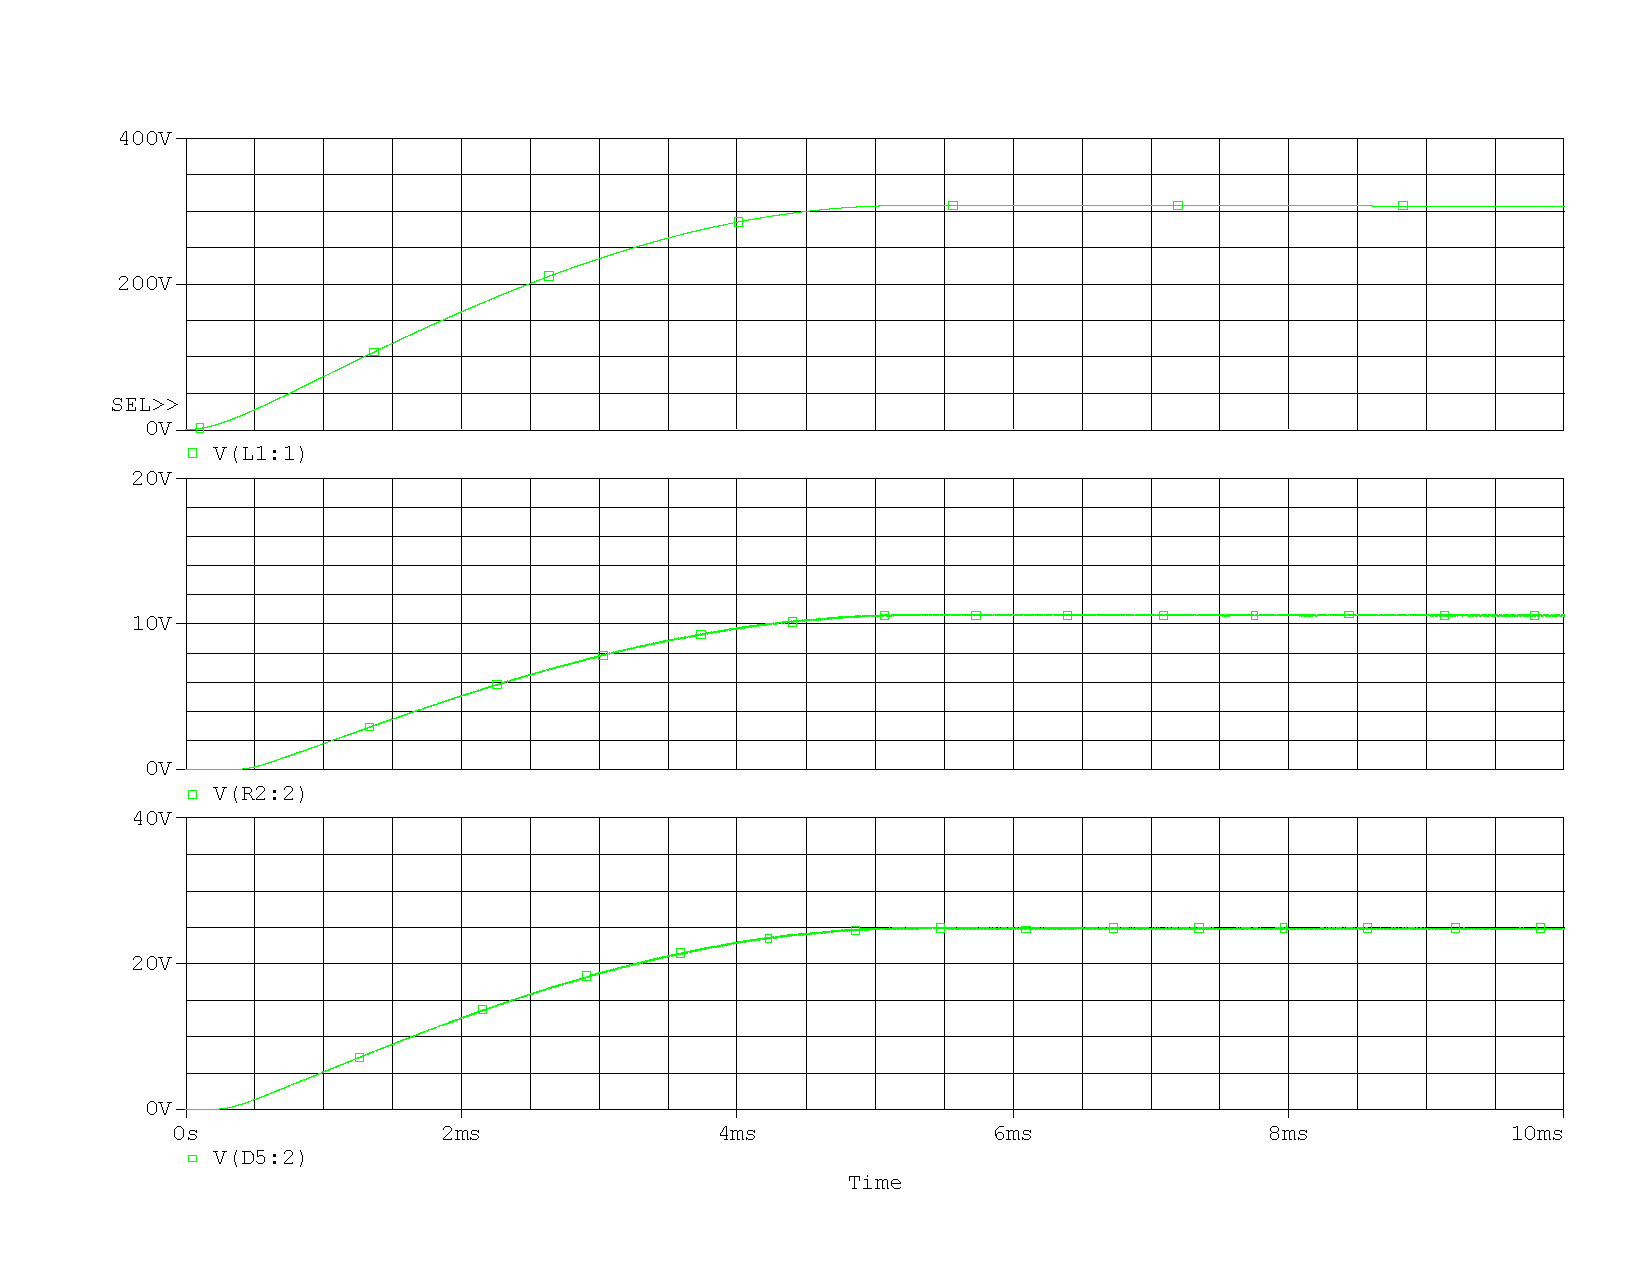
\includegraphics[scale=0.5]{Figuras/1_transitorio_con_rectificador.pdf}
	\caption{Transitorio.}
	\label{fig:transitorio}
\end{figure}

\begin{figure}[H]
	\centering
	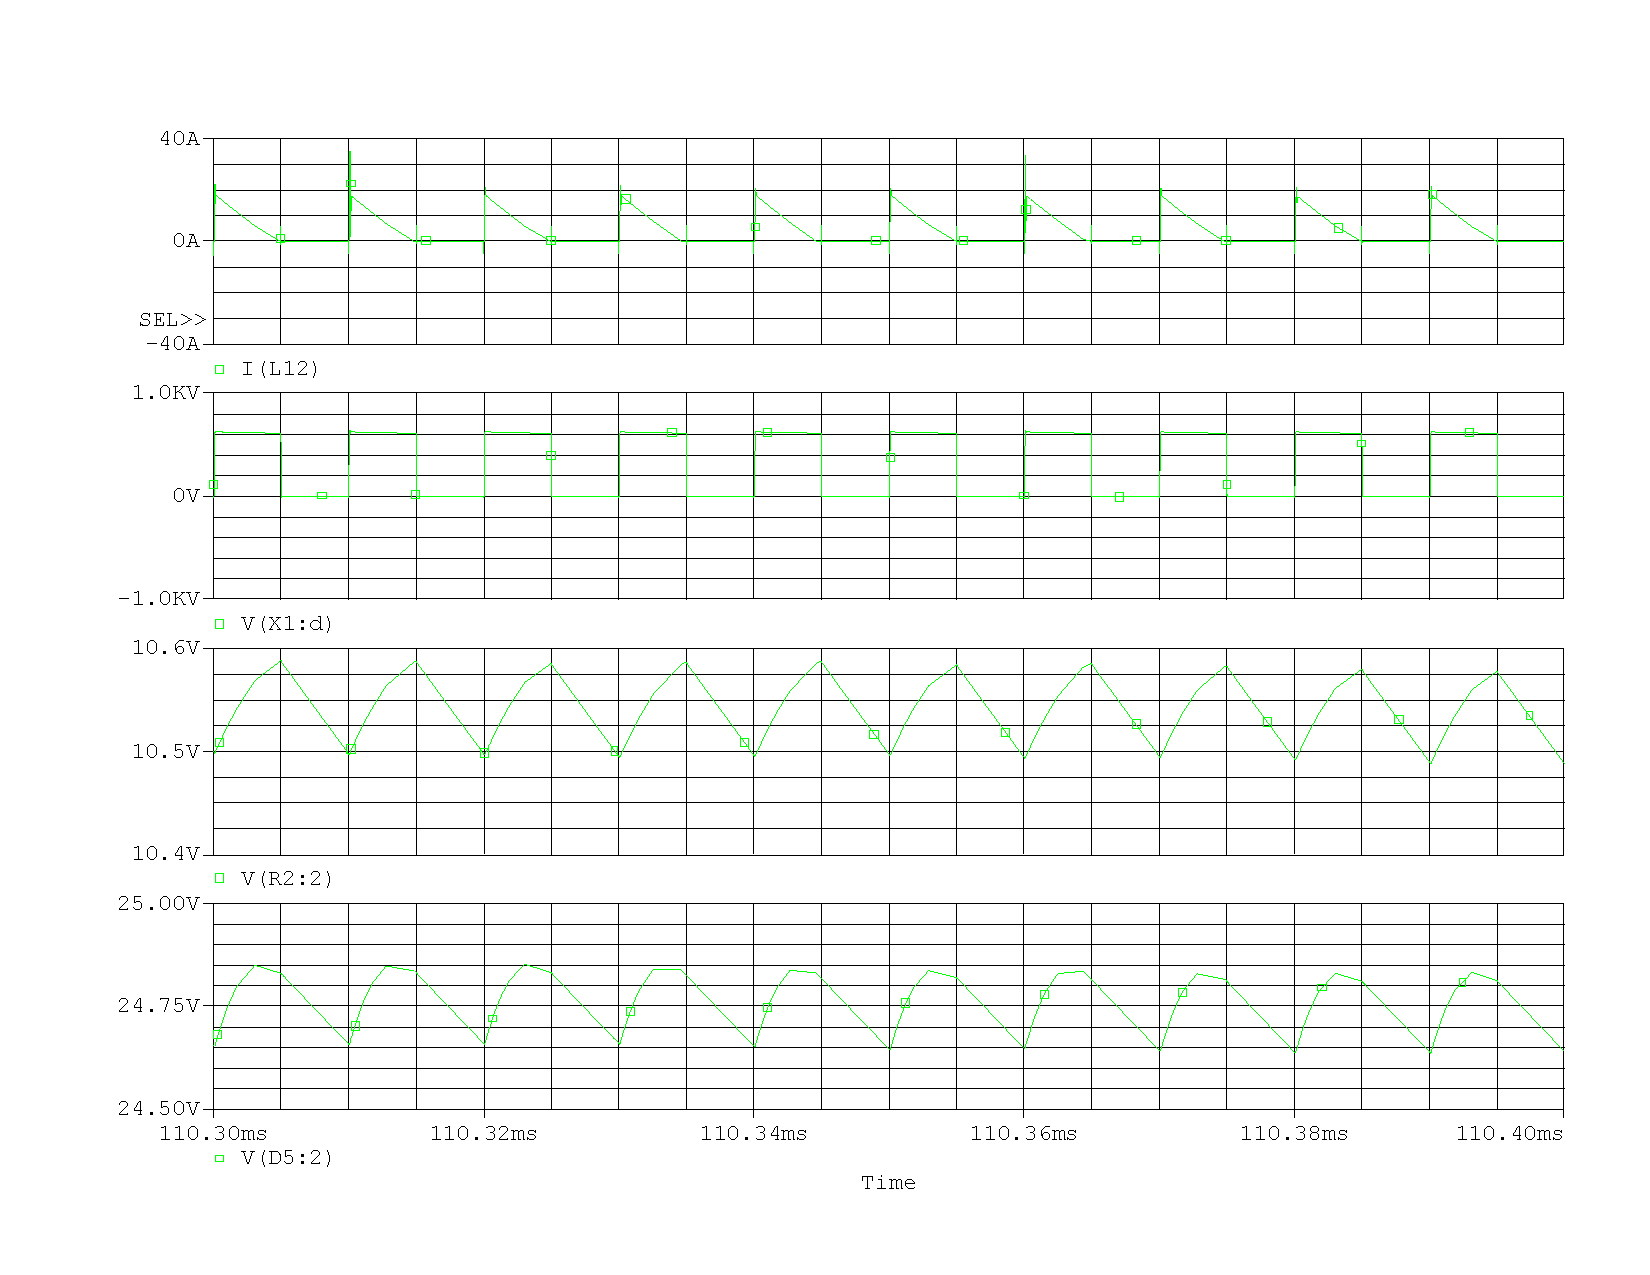
\includegraphics[scale=0.5]{Figuras/1_regimen_permanente.pdf}
	\caption{Régimen permanente.}
	\label{fig:permanente}
\end{figure}


